\documentclass{article}
\usepackage[utf8]{inputenc}
\usepackage{amsmath}
\usepackage{amsfonts}
\usepackage[margin=0.7in]{geometry}
\usepackage{graphicx}
\usepackage{amssymb}
\usepackage{gensymb}
\usepackage{booktabs}
\usepackage{wrapfig}
\usepackage{caption}
\usepackage[export]{adjustbox}
\usepackage[pdfborder={0 0 0}]{hyperref}
\usepackage{pdfpages}
\usepackage{fancyhdr}
\usepackage{parskip}
\usepackage{lastpage}
\usepackage{listings}
\usepackage{multirow}
\usepackage{xifthen}
\usepackage{xcolor}
\usepackage{mathtools}
\graphicspath{{images/}}
\pagestyle{fancy}

\begin{document}
\title{ØkIntro Aflevering 1}
\author{Carl-Emil Rohde - kvb125}
\date{December 2022}
\maketitle

\section{Opgave 1}
\subsection{}
Jeg indsætter værdierne for priserne $p_1$ og $p_2=2$ og indkomst $m=40$ i ligningen for budgetbetingelsen $p_1x_1+p_2x_2 \leq m$ og får: 
$2x_1+2x_2\leq40$

\begin{center}
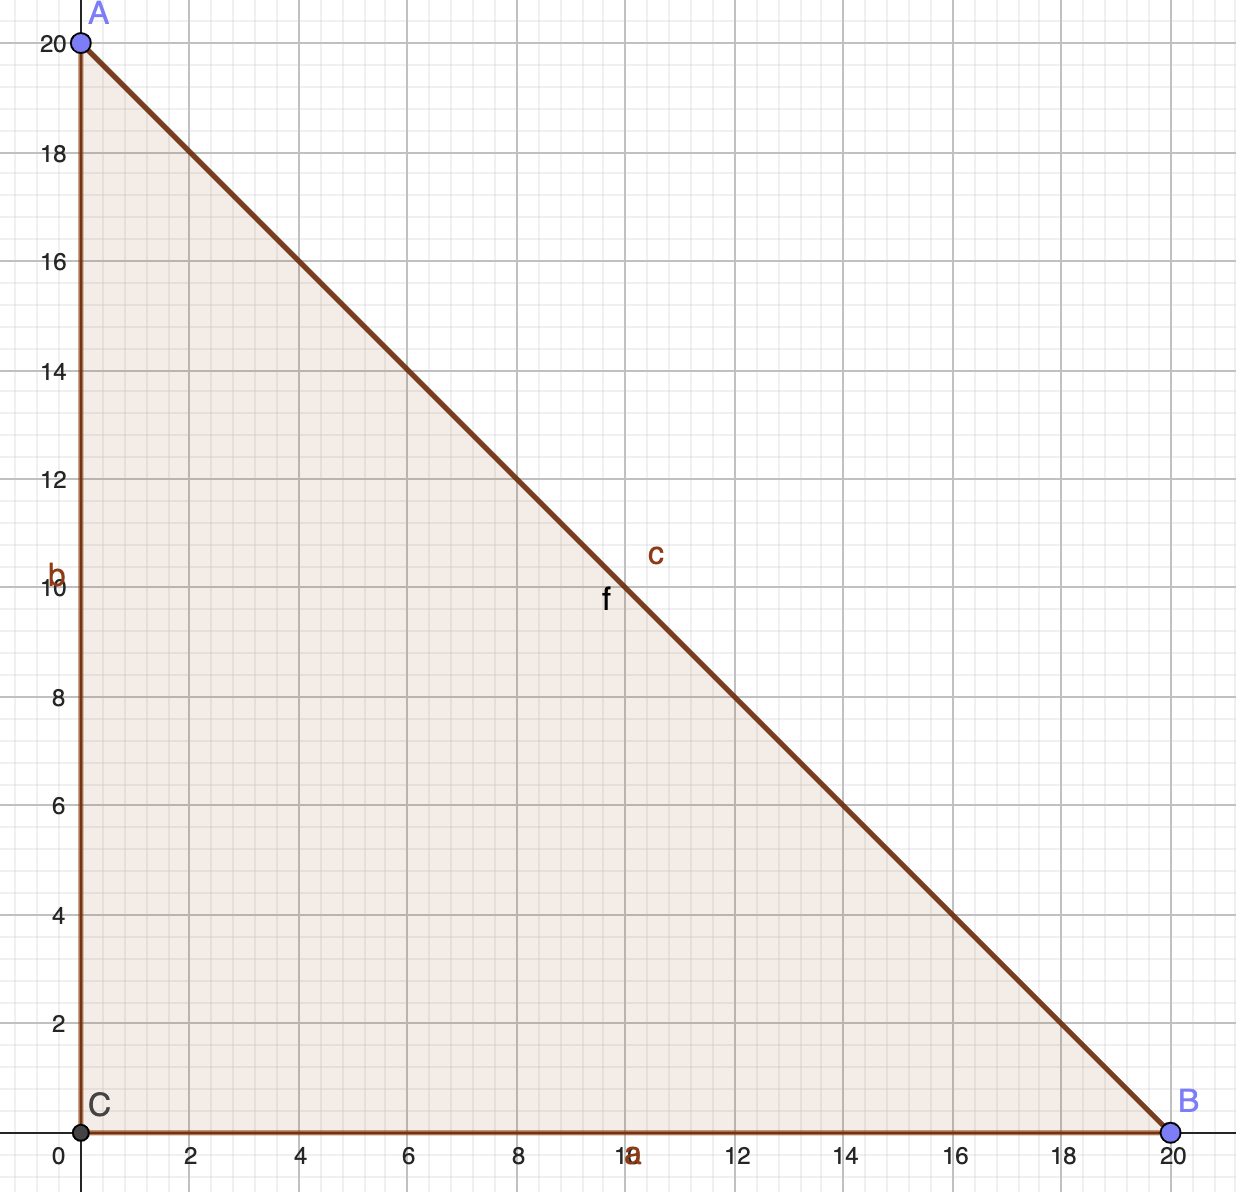
\includegraphics[scale=0.4]{1.png}
\end{center}
På figuren repræsenterer x-aksen gode $x_1$ og y-aksen gode $x_2$. Budgetlinjen har en hældning på $-\frac{P_1}{P_2}=-\frac{2}{2}=-1$

\subsection{}
For at finde ud af hvor meget forbrugeren kan købe af vare 1 og 2, dividerer jeg indkomst med pris. For vare 1: 
$\frac{m}{P_1}=\frac{40}{2}=20$ og for vare 2: $\frac{m}{P_2}=\frac{40}{2}=20$. Den maksimale mængde der kan købes af begge vare er altså 20.

\subsection{}
Jeg opstiller en ny budgetbetingelse med de nye priser, ved at indsætte i formlen for budgetbetingelsen: $p_1x_1+p_2x_2\leq m$ og får: 
$4x_1+2x_2\leq40$

\begin{center}
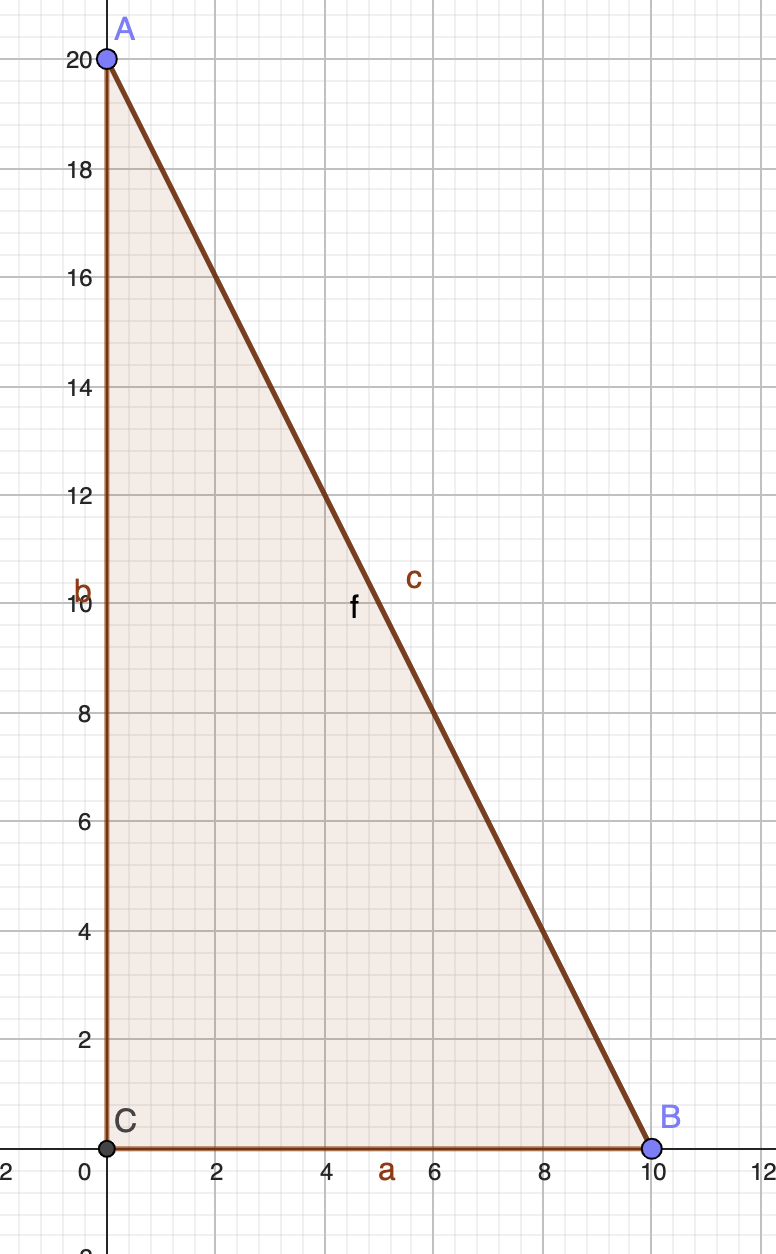
\includegraphics[scale=0.4]{2.png}
\end{center}

På figuren repræsenterer x-aksen gode $x_1$ og y-aksen gode $x_2$. Budgetlinjen har en hældning på $-\frac{P_1}{P_2}=-\frac{4}{2}=-2$

\section{Opgave 2}
\subsection{}
Først starter jeg med at udregne nytten for bundtet (2,4) :

\begin{equation}
    u(2,4)=2*4^\frac{1}{2}=4
\end{equation}

Det samme gør jeg for bundtet (2,16) :
\begin{equation}
    u(2,16)=2*16^\frac{1}{2}=8
\end{equation}

For at finde indifferenskurverne, sætter jeg nytten lig med nyttefunktionen og isolerer for $x_2$.

Først for bundtet (2,4):

\begin{equation}
    x_1x_2^\frac{1}{2}=4
\end{equation}
\begin{equation}
    x_2^\frac{1}{2}=\frac{4}{x_1}
\end{equation}
\begin{equation}
    x_2=(\frac{4}{x_1})^2
\end{equation}
og for bundtet (2,16):
\begin{equation}
    x_1x_2^\frac{1}{2}=8
\end{equation}
\begin{equation}
    x_2^\frac{1}{2}=\frac{8}{x_1}
\end{equation}
\begin{equation}
    x_2=(\frac{8}{x_1})^2
\end{equation}

Nu plotter jeg indifferenskurverne i GeoGebra

\begin{center}
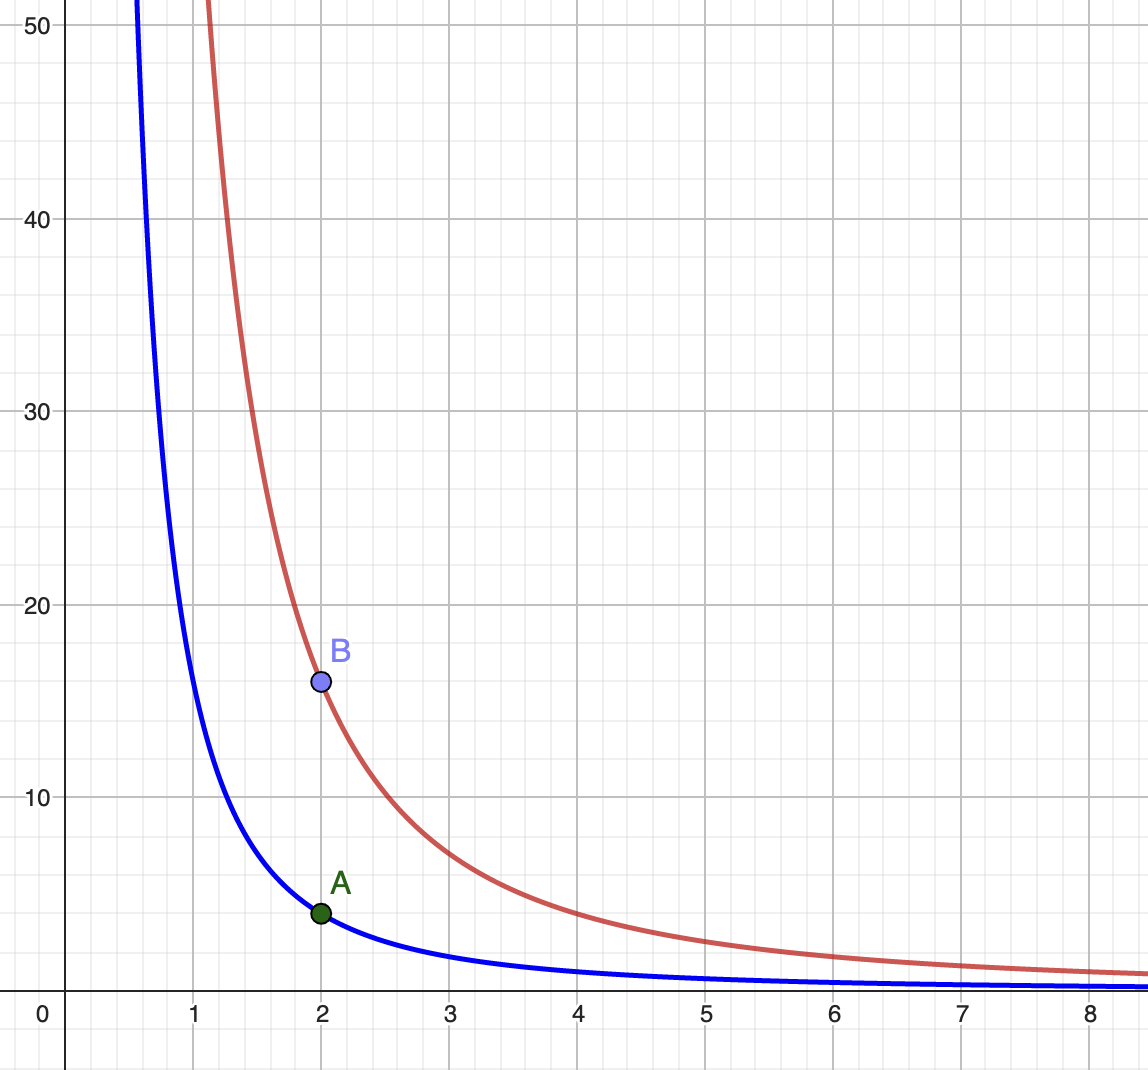
\includegraphics[scale=0.5]{3.png}
\end{center}
Den røde linje repræsenterer alle de bundter, hvor forbrugeren er indifferent fra bundtet (2,16). Den blå for bundtet (2,4).

\subsection{}
For forbruger 2 gør jeg præcis det samme som forbruger 1.

Udregner nytte for bundtet (2,4):
\begin{equation}
    u(2,4)=ln(2)+\frac{1}{2}ln(4)=ln(4)
\end{equation}
Og for bundtet (2,16):
\begin{equation}
    u(2,16)=ln(2)+\frac{1}{2}ln(16)=ln(8)
\end{equation}
Finder indifferenskurver, først for (2,4):
\begin{equation}
    ln(x_1)+\frac{1}{2}ln(x_2)=ln(4)
\end{equation}
\begin{equation}
    \frac{1}{2}ln(x_2)=ln(4)-ln(x_1)
\end{equation}
\begin{equation}
    ln(x_2)=ln(4^2)-ln(x_1)
\end{equation}
\begin{equation}
    x_2=e^{ln(16)}-e^{ln(x_1^2)}
\end{equation}
\begin{equation}
    x_2=e^{ln(16)-ln(x_1^2)}
\end{equation}
Og så for (2,16):
\begin{equation}
    ln(x_1)+\frac{1}{2}ln(x_2)=ln(8)
\end{equation}
\begin{equation}
    \frac{1}{2}ln(x_2)=ln(8)-ln(x_1)
\end{equation}
\begin{equation}
    ln(x_2)=ln(8^2)-ln(x_1^2)
\end{equation}
\begin{equation}
    x_2=e^{ln(64)}-e^{ln(x_1^2)}
\end{equation}
\begin{equation}
    x_2=e^{ln(64)-ln(x_1^2)}
\end{equation}
Nu plotter jeg kurverne i GeoGebra:

\begin{center}
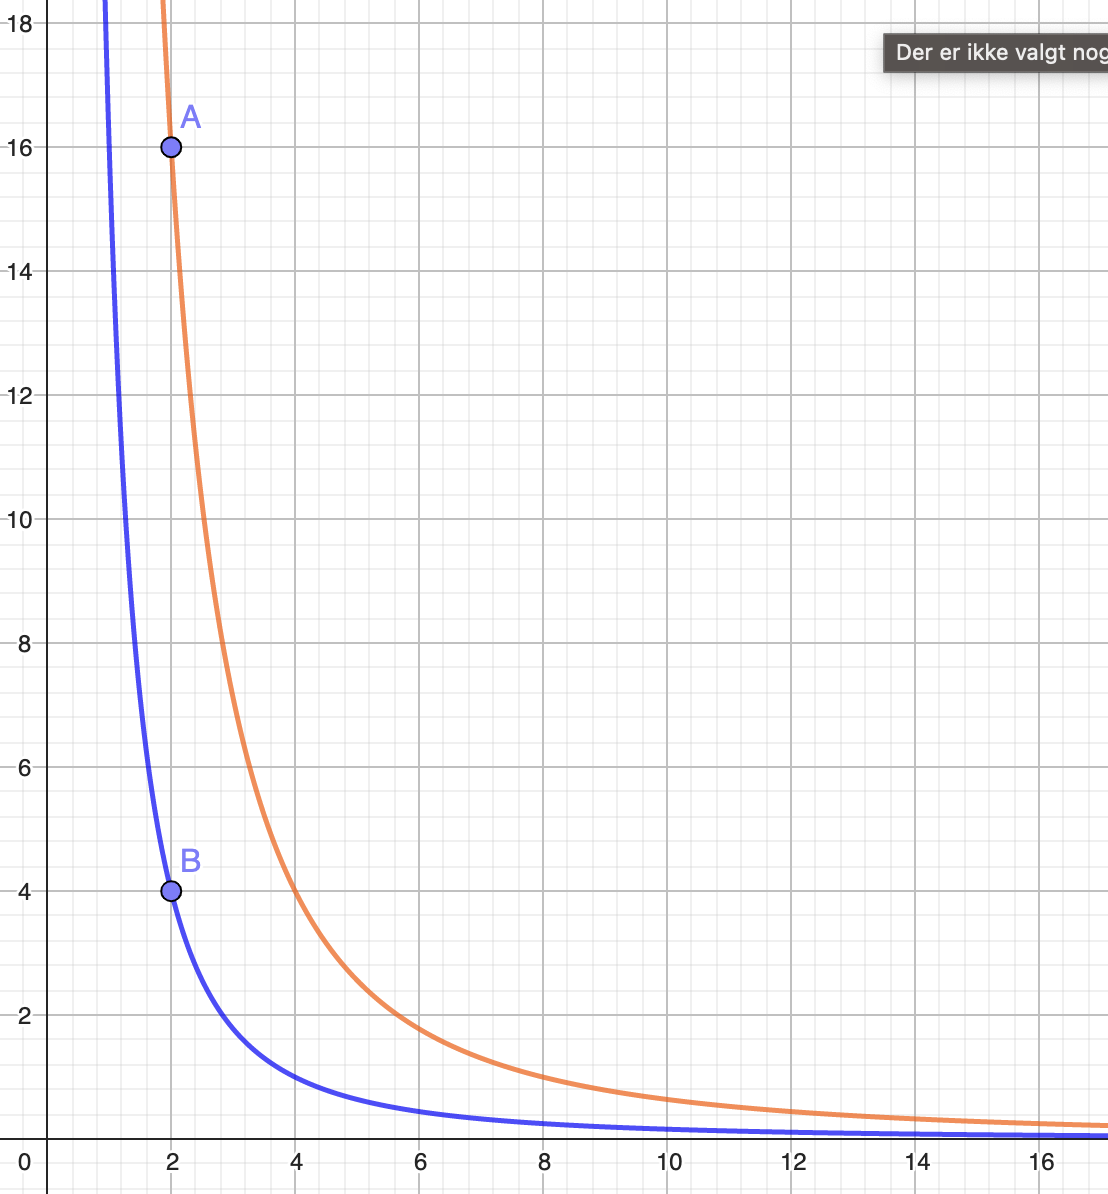
\includegraphics[scale=0.5]{4.png}
\end{center}
Den orange linje repræsenterer alle de bundter, hvor forbrugeren er indifferent fra bundtet (2,16). Den blå for bundtet (2,4).

\subsection{}
Det fremgår af indifferenskurverne, at forbruger 1 og 2 har de samme præferencer. Kurven for bundtet (2,4) er identisk for begge forbrugere, ligegledes for bundtet (2,16). Forbrugerne er altså indifferent imellem de samme bundter, og rangerer dem på samme måde, på trods af at nytten de hver især modtager, ikke er den samme. Begge forbrugere foretrækker bundtet (2,16), da den samlede nytte her er større. Der må altså her være tale om, at forbruger 2's nyttefunktion $u_2$ er en monoton transformation af forbruger 1's nyttefunktion $u_1$. For at bekræfte dette, tjekker jeg om $u_2(x_1,x_2)=g(u_1(x_1,x_2))$:
\begin{equation}
    4 = x_1x_2^\frac{1}{2}
\end{equation}
\begin{equation}
    ln(4)=ln(x_1x_2^\frac{1}{2}
\end{equation}
\begin{equation}
    ln(4)=ln(x_1)+ln(x_2^\frac{1}{2})
\end{equation}
\begin{equation}
    ln(4)=ln(x_1)+\frac{1}{2}ln(x_2)
\end{equation}

Det kan hermed bekræftes, at $u_2$ er en monoton transformation af $u_1$

\subsection{}
For at bestemme om forbrugerne har strengt konvekse præferencer, isoleres $x_2$ i forbruger 1's nyttefunktion, hvorefter jeg finder den dobbeltafledte. Da jeg lige har konkluderet, at begge forbrugere har samme præferencer, kan jeg nøjes med at gøre dette for den ene forbrugers nyytefunkiton. Når jeg differentierer, sætter jeg nytten u=1
\begin{equation}
    u=x_1x_2^{\frac{1}{2}}
\end{equation}
\begin{equation}
    x_2^{\frac{1}{2}}=\frac{u}{x_1}
\end{equation}
\begin{equation}
    x_2=(\frac{u}{x_1})^2
\end{equation}
\begin{equation}
    \frac{dx_2}{dx_1}=2*\frac{1}{x_1}*-\frac{1}{x_1^2}=\frac{-2}{x_1^3}
\end{equation}
\begin{equation}
    \frac{d^2x_2}{d^2x_1}=\frac{0*x_1^3-(-2)*3x_1^2}{(x_1^3)^2}=\frac{6x_1^2}{x_1^6}=\frac{6}{x_1^4}
\end{equation}

Under forudsætning, at $x_1$ og u altid er postive, vil dette udtryk altid være større end 0. Derfor er forbrugernes præferencer strengt konvekse. 

\subsection{}
Det oplyses at $g(z)$ er en strengt monoton funktion. Dette betyder at rangeringen af goderne ikke ændrer sig og at forbruger 1 og 3, derfor burde have de samme præferencer. For at påvise dette, udledes MRS for begge udtryk:
$$
\begin{aligned}
& M R S_1=\frac{\frac{\partial u_1}{\partial x_1}}{\frac{\partial u_1}{\partial x_2}}=\frac{x_2^{\frac{1}{2}}}{x_1 \frac{1}{2} x_2^{\frac{-1}{2}}}=\frac{x_2}{\frac{1}{2} x_1} \\
& M R S_1=\frac{g^{\prime}\left(x_1 * x_2\right) * x_2^{\frac{1}{2}}}{g^{\prime}\left(x_1 * x_2^{\frac{1}{2}}\right) * x_1 * \frac{1}{2} * x_2{ }^{\frac{-1}{2}}}=\frac{x_2}{\frac{1}{2} x_1}
\end{aligned}
$$
$MRS_1$ og $MRS_2$ er identiske. Meget tyder altså på, at forbruger 1 og 3 har samme præferencer. For at være sikker på, at præferencerne er identiske, skal der gælde at funktionerne rangerer bundter på samme måde. Opskrevet matematisk, vil det sige $u_1(x_1,x_2)>u_1(y_1,y_2)$ og $v(x_1,x_2)>v(y_1,y_2)$. Jeg ved fra opgavebeskrivelsen, at $v(x_1,x_2)=g(u_1(x_1,x_2))$, hvilket må betyde at $g(z)$ er en strengt monoton og voksende funktion. Derfor må gælde: $u_1>u_2 \rightarrow g(u_1)>g(u_2)$. Så hvis $u_1(x_1,x_2)>u_2(y_1,y_2)$, vil der gælde at $g(u_1)$ rangerer bundterne identisk, hvilket vil sige at forbrugerne har identiske præferencer. 

\section{Opgave 3}
\subsection{}
Monotone præferencer betyder, at forbrugerens nytte stiger, hvis mængden af goder stiger. Hvis dette er tilfædet, skal den første afledte af nyttefunktionen $u(x_1,x_2)=x_1^2x_2$ med hensyn til både $x_1$ og $x_2$ være postiv. Jeg udregner: 
\begin{equation}
    \frac{du}{dx_1}=2x_1x_2
\end{equation}
og
\begin{equation}
    \frac{du}{dx_2}= x_1^2
\end{equation}
Begge udtryk er positive, så det kan konkluderes, at forbrugeren har monotone præferencer. For at finde ud af om forbrugeren har strengt konvekse præferencer, isolerer jeg $x_2$ i nyttefunktionen og finder den dobbeltafledede. Hvis den er positiv, er præferencerne konvekse. 

\begin{equation}
    u=x_1^2x_2
\end{equation}
\begin{equation}
    x_2=\frac{u}{x_1^2}
\end{equation}
\begin{equation}
    \frac{dx_2}{dx_1}=\frac{0*x_1^2-u*2x_1}{(x_1^2)^2}=\frac{-2x_1u}{x_1^4}=\frac{-2u}{x_1^3}
\end{equation}
\begin{equation}
    \frac{d^2x_2}{d^2x_1}=\frac{0*x_1^3-(-2u)*3x_1^2}{(3x_1^2)^2}=\frac{6}{x_1^4}
\end{equation}
Den første afledte er negativ og den anden afledte er positiv. Derfor er præferencerne strengt konvekse. 

Nu opstiller og løser jeg forbrugerens problem ved brug af lagrange:
\begin{equation}
    L(x_1,x_2,\lambda)=x_1^2x_2-\lambda(p_1x_1+p_2x_2-m)
\end{equation}
Partiel differentiering for alle variable:
\begin{equation}
    1) \frac{dL}{dx_1}=2x_1x_2-\lambda p_1=0
\end{equation}
\begin{equation}
    2) \frac{dL}{dx_2}=x_1^2-\lambda p_2=0
\end{equation}
\begin{equation}
    3) \frac{dL}{d\lambda}=-p_1x_1-p_2x_2+m=0 <=> m=p_1x_1+p_2x_2=0
\end{equation}
Isoler $\lambda$ i ligning (1):
\begin{equation}
    2x_1x_2-\lambda p_1=0
\end{equation}
\begin{equation}
    2x_1x_2=\lambda p_1
\end{equation}
\begin{equation}
    \lambda = \frac{2x_1x_2}{p_1}
\end{equation}
Indsæt $\lamdda$ i ligning (2) og find $x_1$
\begin{equation}
    x_1^2-\frac{2x_1x_2}{p_1}p_2=0
\end{equation}
\begin{equation}
    x_1^2=\frac{2x_1x_2p_2}{p_1}
\end{equation}
\begin{equation}
    x_1=\frac{2x_2p_2}{p_1}
\end{equation}
Indsæt $x_1$ i ligning (3) og find $x_2$
\begin{equation}
    m=p_1\frac{2x_2p_2}{p_1}+p_2x_2
\end{equation}
\begin{equation}
    m=2x_2p_2+p_2x_2
\end{equation}
\begin{equation}
    x_2=\frac{m}{3p_2}
\end{equation}
Indsæt $x_2$ i ligning (3) og find $x_1$
\begin{equation}
    m=p_1x_1+p_2\frac{m}{3p_2}
\end{equation}
\begin{equation}
    m=p_1x_1+\frac{m}{3}
\end{equation}
\begin{equation}
    m-\frac{m}{3}=p_1x_1
\end{equation}
\begin{equation}
    x_1=\frac{2m}{3p_1}
\end{equation}
Således er forbrugerens efterspørgselsfunktioner $x_1=\frac{2m}{3p_1}$ og $x_2=\frac{m}{3p_2}$

\subsection{}
Hvis gode $x_1$ skal være et normalt gode, skal der gælde: $\frac{dx_1}{dm}>0$. Jeg differentierer $x_1$ med hensyn til m:
\begin{equation}
    \frac{dx_1}{dm}=\frac{2}{3p_1}
\end{equation}
Den afledte med hensyn til indkomst er positiv. Derfor er gode $x_1$ et normalt gode. Hvis godet skulle have været inferiørt, skulle den afledte have været negativ. Hvis gode $x_1$ er ordinært, skal den afledte af $x_1$ med hensyn til $p_1$ være negativ:
\begin{equation}
    \frac{dx_1}{dp_1}= \frac{-2m}{3p_1^2}
\end{equation}
Udtrykket er negativt, derfor er der tale om et ordinært gode og ikke et giffen gode. Hvis goder er substitutter eller komplimenter, har en ændring i pris på det ene gode, en effekt på efterspørgslen på det andet gode. For at finde ud af om denne sammenhæng er til stede, differentirerer jeg efterspørgselsfunktionen for begge goder, med hensyn til prisen på det modsatte gode:

$$
\frac{\partial \mathrm{x}_1}{\partial \mathrm{p}_2}=\frac{\partial\left(\frac{2m}{3 p_1}\right)}{\partial \mathrm{p}_2}=0
$$
og
$$
\frac{\partial \mathrm{x}_2}{\partial P_1}=\frac{\partial\left(\frac{m}{3 p_2}\right)}{\partial \mathrm{p}_1}=0
$$
Begge disse udtryk giver 0, hvilket må betyde at goderne hverken er substitutter eller komplementer. 


\subsection{}
For at vurdere effekten af en stykskat, udregner jeg først forbrugerens nytte uden stykskat:
\begin{equation}
    x_1=\frac{2*3}{3*1}=\frac{6}{3}=2
\end{equation}
\begin{equation}
    x_2=\frac{3}{3*1}=1
\end{equation}
\begin{equation}
    u(2,1)=2^2*1=4
\end{equation}
Nu udregner jeg nytten efter $x_1$ pålægges en stykskat på 1, hvilket vil sige $p_1$ nu er 2. 
\begin{equation}
    x_1=\frac{2*3}{3*2}=\frac{6}{6}=1
\end{equation}
\begin{equation}
    x_2=\frac{3}{3*1}=1
\end{equation}
\begin{equation}
    u(1,1)=1^2*1=1
\end{equation}
Før stykskat, havde forbrugeren altså en nytte på 4. Efter stykskat en nytte på 1. Stykskatten har derfor en negativ effekt på forbrugerens nytte. For at finde ud af, hvor meget staten får ind i skatteindtægter, kan vi gange mængden af gode $x_1$ der forbruges, med stykskatten. Staten tjener altså $R=t*x_1=1*1=1$ krone i skatteindtægt.

\subsection{}
For at finde ud af, hvor meget staten kan få ud af at ændre stykskatten til en indkomstskat, opstiller jeg et udtryk hvor jeg indsætter efterspørgselsfunktionerne for $x_1$ og $x_2$ i forbrugerens nyttefunktion. Jeg indfører $T$, som er indkomstskatten der trækkes fra indkomsten. Jeg indsætter priserne $p_1$ og $p_2$, samt indkomsten $m$:
$$
u\left(x_1, x_2 \right)=\left(\frac{2(m-T)}{3 p_1}\right)^2 * \frac{m-T}{3 p_2}=\left(\frac{2 *(3-T)}{3 * 1}\right)^2 * \frac{3-T}{3 * 1}
$$
Dette udtryk sætter jeg lig med 1, da forbrugeren skal forblive indifferent: 
$$
\left(\frac{2 *(3-T)}{3 * 1}\right)^2 *\left(\frac{3-T}{3 * 1}\right)=1
$$
Dette ligningssystem, løser jeg nu for $T$:

\begin{equation}
    \frac{(2(3-t))^2}{3^2}*\frac{(3-T)}{3}=1
\end{equation}
\begin{equation}
    \frac{2^2(3-T)^2}{9}*\frac{(3-T)}{3}=1
\end{equation}
\begin{equation}
    \frac{4(3-T)^3}{27}=1
\end{equation}
\begin{equation}
    4(3-T)^3=27
\end{equation}
\begin{equation}
    (3-T)^3=\frac{27}{4}
\end{equation}
\begin{equation}
    3-T=\sqrt[3]{\frac{27}{4}}
\end{equation}
\begin{equation}
    -T=\sqrt[3]{\frac{27}{4}}-3
\end{equation}
\begin{equation}
    T=-\sqrt[3]{\frac{27}{4}}+3
\end{equation}
\begin{equation}
    T\approx1,1
\end{equation}
Det fremgår altså, at ved at skifte til en indkomstskat, kan forbrugeren forblive indifferent, samtidig med at staten øger sin skatteindtægt, da $T>1$. En indkomstskat er derfor at foretrække. Dette er fordi, stykskatten forvridder forbrugerens efterspørgsel i højere grad end indkomstskatten. Som et resultat af stykskatten, køber forbrugeren mindre af $x_1$, hvilket sænker skatteindtægter. Man kan sige, at forbrugerens elasticitet i forhold til forbrug, er højere end i forhold til arbejde. Alt i alt, er indkomstskatten i det her tilfælde altså en bedre løsning. 
\end{document}


